% !TEX root = ../main.tex
%
\chapter{The (end of the) monocentric city}
\label{chap:monocentric_introduction}

\begin{flushright}{\slshape    
It may be a small irony that  
just as\\
the phenomenon of polycentricity\\ is getting considerable attention,\\
The world is moving beyond it.} \\ \medskip
--- Peter Gordon \& Harry Richardson~\cite{Gordon:1996}
\end{flushright}

The hypothesis that cities organise themselves around a single center of
activities---the Central Business District in the US---may well be one of the
strongest hypothesis in urban studies. Although no one seriously believes in its
validity any more, its influence is still creeping, often unnoticed, in many
empirical and theoretical works.  In order to deconstruct the monocentric model,
we first need to understand where it came from in the first place, for what
reason it was introduced and what evidence it was based on. In this chapter, we
present a historical perspective on the monocentric hypothesis: the context in
which it was introduced, and how it was gradually realised that cities had a
decentralised structure. We will end with a review of the emergence of the
notion of center and of the tools developed to measure their number.

\section{From monocentric, to polycentric and dispersed cities}
\label{sec:introduction}

Maybe the least assuming way to represent the density profiles in cities is
through cloropleth maps or 3-dimensional representation where the $x$ and $y$
coordinates correspond to the original coordinates projected on the plane, and
the $z$ coordinate to the density. The former approach can be traced back as far
as $1898$ with Meunot's \emph{Des agglom\'erations urbaines dans l'Europe
contemporaine}~\cite{Meunot:1898} who drew a large number of density maps of
large Europen cities, later followed by Jefferson in
$1909$~\cite{Jefferson:1909} who did the same for several cities in the US,
Europe and Australia. On Fig.~\ref{fig:density_3d} we use the latter approach to
represent density profiles for two metropolitan areas in the US: Minneapolis-St.
Paul and Houston. \\


\begin{figure}
    \centering
    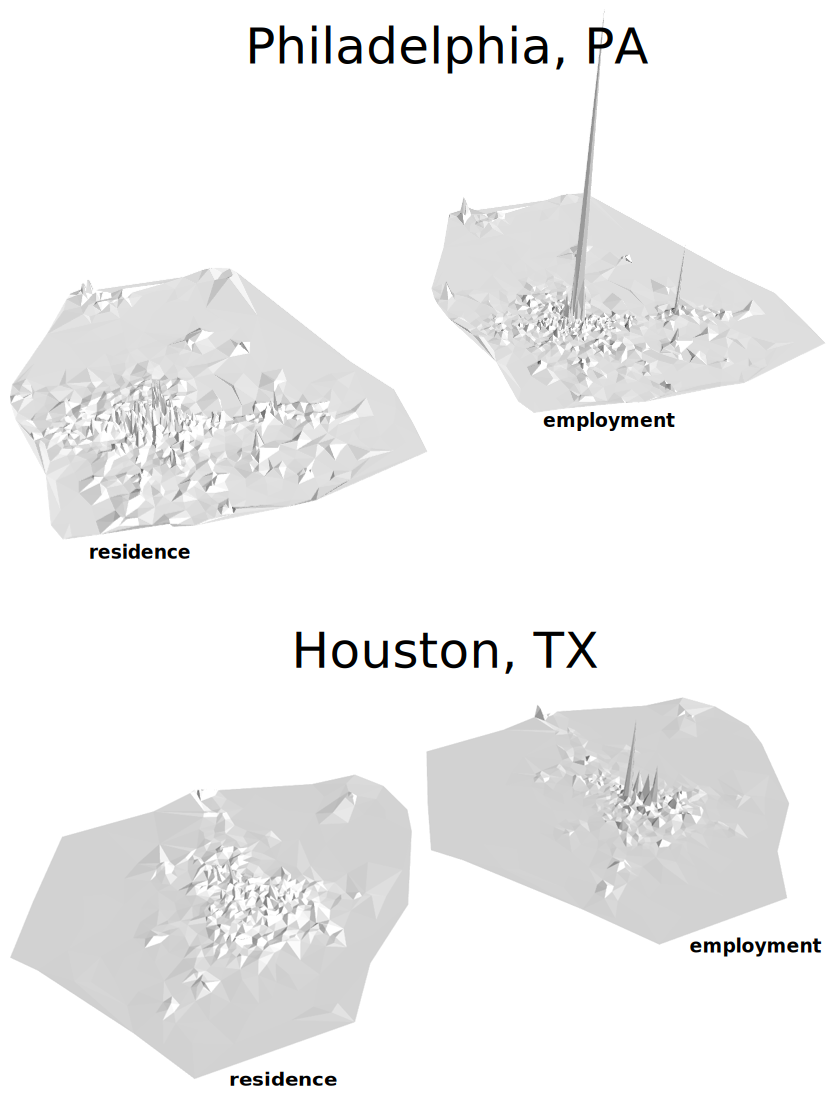
\includegraphics[width=\textwidth]{gfx/chapter-monocentric/panel_3d.png}
    \caption{{\bf 3D representations of densities.} (Top) The Metropolitan
        Statistical Area (MSA) of Philadelphia, PA. (Bottom) The MSA of Houston,
    TX. Employment and Population densities are plotted at the same scale.
Employment densities are sensibly more peaked than employment densities, making
the notion of `center' more intuitive. Data were obtained from the 2000 US
Census; the figures were prepared with Python and Inkscape.
\label{fig:density_3d}}
\end{figure}


These two cities are enough to get an idea of the difficulties associated with
studying density profiles.
First comes the question of what densities we are talking about. Indeed, people
are constantly moving throughout the city, and density profiles can only be
(approximate) snapshots of the city at different instants during the day.
Traditionally -- because of the availability of data -- people have mainly
considered the residence and employment density. This roughly gives an idea of
the densities in the city at night and during the day, and can thus help
understand the commuting patterns. We note that the availability of mobile phone
data that are continous in time might help to give a more precise, almost
real-time, and continuous picture of the densities during the
day~\cite{Louail:2014}.\\

Then comes the problem of how to makes sense of these patterns. The densities
represented on Fig.~\ref{fig:density_3d} are indeed very complex, and it would
help their understanding if we could isolate some particular structure.
This is what Clark did in $1951$~\cite{Clark:1951}. Realising that (1) districts of large
population tend to be in the interior, districts of small population in the
exterior (2) as cities expand, they tend to spread themselves out, he proposes
to write the density $\rho$ as a function of the distance $d$ from the center

\begin{equation}
    \rho = a\,e^{-d/b} 
\end{equation}

And, to justify his assumption, plots the population density of various cities as a function of
the distance to the center~\cite{Clark:1951}. The monocentric hypothesis was
born.

Looking at the density profiles plotted by Clark in 1951~\cite{Clark:1951} for
many cities across the world, or on Fig.~\ref{fig:distance_center_minneapolis}
for the Metropolitan Statistical Area of Minneapolis, one can be
forgiven for thinking that cities have a monocentric structure. Such profiles
indeed almost always exhibit a sharp decrease as we go farther from the city
center -- defined as the areal unit with the highest density. However, this
pattern is only the signature of a monocentric pattern if one makes the further
hypothesis that the pattern of employment densities in cites are symmetric
under rotations around the center. Obviously, this is not the case: cities are
nowhere isotropic but in the imagination of modelers.


\begin{figure}
    \centering
    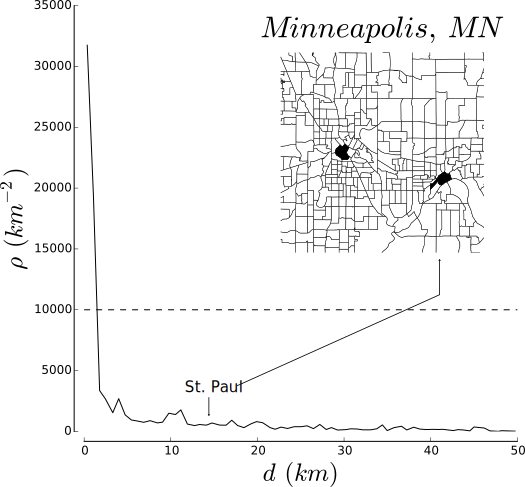
\includegraphics[width=\textwidth]{./gfx/chapter-monocentric/distance_center_minneapolis.pdf}
    \caption{Employment density as a function of distance to the center for the
    Metropolitan Statistical Area of Minneapolis-St. Paul in 2000. The center is defined here as the
    tract with the highest employment density, and corresponds to the historical
    Central Business District of Minneapolis. The curve exhibits a very sharp
    decay, giving the illusion of a monocentric structure. (Inset) The census tracts
    of Minneapolis-St. Paul in 2000. In black, the census tracts where the
    employment density reaches values above $10,000\,\text{km}^{-2}$. The two tracts
    coincide with the historical centers of the Twin Cities, and are distant from
    $14\,\text{km}$. This fragmented structure cannot be infered from the density
    profile on the left (arrow on the curve).
    \label{fig:distance_center_Minneapolis}}
\end{figure}


So why did Clark's methods and plots did not become a simple curiosity, but were
instead so widely adopted? Although we cannot explain why such and such and
things happened, there is little doubt that the echo this idea had in urban
economics has something to do with it. From an implied assumption in an empirical analyis, the monocentric hypothesis
only became clearly stated with the theoretical work of
economists.\cite{Muth:1969} Model showing how we could obtain.



The Alonso-Muth-Mills model might well be the reason for the long-lasting influence of
the monocentric model (a nice exposition of the model can be found
in~\cite{Fujita:1989}). In 1964, Alonso introduced the bid-rent curve as a
function of the distance to the city center~\cite{Alonso:1964}. The simplifying hypothesis of
\emph{monocentricity} naturally followed, the assumption that all firms in a
city are concentrated in a single, fixed-size part of the city, the central business
district. We should not underestimate how this model influenced many people's
perception of what a city is. In the US, the name of Central Business District
is casually used as a way to designate the principle activity center in a city.
Many, if not most, measures of the spatial variation of quantities inside cities
actually use the notion of `distance to the city center'. This only makes sense,
however, under the assumption of monocentricity. Most of the
literature has not departed from the monocentric assumption---sometimes without
being aware of it! In the defense of these authors however, there is a clear
lack of appropriate tools to study spatial profiles.


\cite{Mills:1972} is a monograph discussing the causes of decentralisation and
suburbanisation. [could not read]

\cite{Kemper:1974} explores data trying to fit a negative exponential function
to industry and employment density. It does not work so well.

\cite{Odland:1978} explores the possibility of polycentric cities on a
theoretical basis. [could not read]

\cite{Griffith:1981} tool to evaluate the polycentricity of a pattern.[could not
read]

Treatment of the polycentric city in the urban economics literature starts
with~\cite{Fujita:1982}.

In 1987 appear the first measures of the number of centers!


\cite{Dokmeci:1994} shows that Istanbul's employment is spread across several
centers. Although there is still a lack of strong quantitative evidence, the
idea is gaining ground.

\cite{Garreau:1991} Edge cities.

\cite{Gordon:1996} Beyond polycentricity: the dispersed city.

The lesson that should be learned from the article by Gordon and Richardson is
that the notion of polycentricity is \emph{also an hypothesis} on the spatial
structure of densities. While it is arguably more involved than the monocentric
hypothesis, it does indeed consists in imposing some structure onto the raw
data. The process itself of counting centers implies that these centers exist,
that there is an element of reality attached to what we call centers. A quick
look on the 3D plot shown on Fig.~\ref{density_3d} should convince the reader
that the world is not as simple as the way we picture it. While employment
densities indeed exhibit strong peaks that are easily distinguishible (although
that is arguable for Houston), the same cannot be said for population densities.

In the following however, we will work in the framework of the polycentric
assumption (as I have during my thesis). The problems linked with the
simplification will be put aside for a moment and adressed at various stages in
the following.


\section{How to measure polycentrity}
\label{sec:how_to_measure_polycentrity}

\cite{Tsai:2005} is a classic on Urban Form, along with~\cite{LeNechet:2015} and
\cite{Schwarz:2010}.

\cite{McDonald:1987} proposes the first empirical method to identify employment
subcenters.

\cite{Giuliano:1991} uses an arbitrary threshold to determine the centers.

\cite{Anas:1998} Critices the method of Giuliano, has a cool picture of
Los-Angeles spreading and deals with urban structure.

\cite{Bertaud:2001} is very interesting on urban form in general, and proposes
an index, the eccentricity, to measure the distance of the center of gravity to
the geographical CBD.


\cite{McMillen:2001} proposes a non-parametric method to find the subcenters.

\cite{McMillen:2003} proposes a pretty good literature review in introduction on
the identification of employment subcenters, and proposes congestion as a reason
for the polycentric transition.


\cite{Griffith:2007} is yet another reference on spatial regression.\\

\cite{Redfearn:2007} Proposes interesting visualisations and a parametric method
to determinate the number of centers.\\

Have a look at what~\cite{Berroir:2008} do!


\cite{LeNechet:2010} introduces the acentrism index (also explained
in~\cite{LeNechet:2015}.\\

\cite{Pereira:2013} proposes an Urban Centrality Index that varies continuously
between a monocentric configuration and an extreme decentralized situation.

\cite{Louf:2013_polycentric} Proposes to use a property of the rank plot of the
employment density, exponential decrease.

\cite{Louail:2014} proposes a generalisation of the previous method based on the
Lorenz curve.

I propose a generalisation, based on the same hypothesis but that is more robust
than the computation of the tangent at the origin.


\section{The polycentric transition}
\label{sec:the_polycentric_transition}

Justify the term `polycentric transition'. When the population increases, it is
clear that the number of centers increases as well. Therefore, it seems that, as
they grow and expand, urban systems develop a more and more polycentric form.

\subsection{Empirical evidence}
\label{sub:empirical_evidence}


\section{Reasons invoked for the polycentric transition}
\label{sec:reasons_invoked_for_the_polycentric_transition}

We exlude the cases where polycentrism finds its origin in the fusion of two
Metropolises (Copenhagen-Malm\"o, Twin Cities, Ruhr) or through the
incorporation of satellite municipalities.\\


\cite{McMillen:2003} suggests congestion might be the reason for polycentrism.
so does Mills in 1972...

